\documentclass[10pt]{article}
\usepackage{graphicx} % Required for inserting images
\usepackage{geometry}
\usepackage[english,spanish]{babel}
\usepackage{blindtext}
\usepackage{lipsum}
\usepackage{parskip}
\usepackage{setspace}
\usepackage{caption}
\usepackage{multicol}
\usepackage{hyperref}
\usepackage{float}
\usepackage{changepage}
\usepackage{longtable}
\usepackage{multirow}
\usepackage{amsmath}
\usepackage{ragged2e}
\usepackage{graphicx}
\usepackage[style=apa,backend=biber]{biblatex}
\addbibresource{referencias.bib}

\usepackage{parskip}

\usepackage{tikz}

\usetikzlibrary{shapes, arrows}
\usetikzlibrary{shapes.geometric}
\usetikzlibrary{positioning}
\usetikzlibrary{positioning, arrows.meta}
\usetikzlibrary{shapes, arrows.meta}

\tikzstyle{block} = [rectangle, draw, fill=blue!20, text width=6em, text centered, rounded corners, minimum height=3em]
\tikzstyle{line} = [draw, -latex']
\tikzstyle{cloud} = [draw, ellipse, fill=red!20, node distance=3cm, minimum height=2em]

\usepackage{schemata}
\usetikzlibrary{mindmap}

\usetikzlibrary{fit,positioning}

\geometry{
    top=2.5cm,
    left=2.8cm,
    right=2.8cm,
    bottom=2.44cm
}

\tikzset{
every picture/.append style={
  execute at begin picture={\deactivatequoting},
  execute at end picture={\activatequoting}
  }
}

\usepackage{titlesec}

\titleformat{\section}{\fontsize{10}{12}\selectfont\bfseries\centering}{\thesection. }{1em}{}
\titlespacing*{\section}{0pt}{\baselineskip}{\baselineskip}

\titleformat{\subsection}{\fontsize{10}{12}\selectfont \itshape}{\thesubsection. }{1em}{}
\titlespacing*{\subsection}{0pt}{\baselineskip}{\baselineskip}

\titleformat{\subsubsection}{\fontsize{10}{12}\selectfont \itshape}{\thesubsubsection. }{1em}{}
\titlespacing*{\subsubsection}{0pt}{\baselineskip}{\baselineskip}

\usepackage[pages=all]{background}

\backgroundsetup{
 scale=1, %escala de la imagen, es recomendable que sea del mismo tamaño que el pdf
 color=black, %fondo a usar para transparencia
 opacity=0.2, %nivel de transparencia
 angle=0, %en caso de querer una rotación
 contents={%
  \includegraphics[width=\paperwidth,height=\paperheight]{Plantilla Latex CIETA.pdf} %nombre de la imagen a utilizar como fondo
 }%
}

\usepackage{fontspec}
\setmainfont{Times New Roman}

\title{
    \vspace{0mm} \textbf{Computational Politics: Advancing Sentiment Analysis through Natural Language Processing in Election Studies}\vspace{4mm}
}
\author{
    \fontsize{10}{12}\selectfont \textbf{Mundhir AL Bohri}\\ \\
    \small{\textbf{\fontsize{10}{12}\selectfont Dalhousie University}}\\
    \small{\fontsize{10}{12}\selectfont Faculty of Computer Science}\\
    \small{\fontsize{10}{12}\selectfont CSCI 4152/6509 Natural Language Processing}\\
    \small{\fontsize{10}{12}\selectfont Course Instructor: Dr. Vlado Keselj}\\
    \small{\fontsize{10}{12}\selectfont E-mail: mn409130@dal.ca}
}
\date{\vspace{-6mm}}

\begin{document}

\fontsize{10}{12}\selectfont

\selectlanguage{english}

\def\tablename{Tabla}%

\setlength{\parskip}{0mm}

\maketitle

\setlength{\parskip}{3mm}

\selectlanguage{english}

\renewcommand\abstractname{}

\begin{abstract}
    \fontsize{10}{12}\selectfont
    \textbf{Abstract:} This paper examines the application of Natural Language Processing (NLP) for sentiment analysis in the context of political elections, focusing on methodologies such as the Naive Bayes Classifier and advanced transformer models like BERT and LLAMA 2. Our research analyzes social media data, particularly from the 2020 US election, to gain insights into public opinion on political issues. We conduct a comparative study of these NLP techniques to evaluate their effectiveness in interpreting the complexities of political discourse on social media. Our findings reveal notable differences in the performance of these methods, offering valuable perspectives for electoral studies and practical implications for political campaign strategies.

    \vspace{3mm}
    
    \textbf{Keywords:} Sentiment Analysis, Probabilistic Models, Transformer Models.
    \vspace{-7mm}
\end{abstract}

\vspace{8mm}

\setlength{\columnsep}{1cm}

\renewcommand{\tablename}{Tabla}

\begin{multicols}{2}
\fontsize{10}{12}\selectfont

\section{INTRODUCTION}
The integration of Artificial Intelligence (AI) into political campaigns has markedly transformed election strategies and analysis. This is evidenced by the significant impact AI had in the 2016 Trump presidential campaign and the Brexit referendum's U.K. Leave Campaign (\cite{8664495}). While these developments showcase AI's potential in influencing public opinion and election outcomes, they also raise ethical concerns and highlight the challenges in monitoring AI technologies that are proprietary to private corporations. This paper proposes a methodology for engaging critically with AI tools in governance, aiming to enhance integrity and trust in electoral systems.

Our study focuses on the application of Natural Language Processing (NLP) to analyze political discourse on social media platforms. These platforms, rich with public opinions on political subjects, provide an essential resource for understanding societal sentiments. However, efficiently processing this large and complex dataset is a substantial challenge.

Our research emphasizes the use of smaller, more accessible NLP models, especially in settings with limited computational resources. The study begins with the Naive Bayes Classifier as a simple yet effective baseline model and progresses to examine advanced models like BERT (\cite{devlin2018bert}) and LLAMA 2 (\cite{touvron2023llama}), focusing on their fine-tuning to optimize performance. Additionally, we include a comparison with GPT-4 Turbo, based on the GPT-4 but with 128k context window (\cite{openai2023gpt4}), to assess the performance of these smaller models against a more advanced, extensive model in political sentiment analysis.

The dual aims of this research are to utilize smaller NLP models for extracting meaningful insights from online political discussions and to evaluate their performance against the backdrop of advanced models like GPT-4 Turbo. This approach will help us understand the effectiveness and viability of smaller models in the detailed field of political sentiment analysis.

\section{RELATED WORK}

In this section, we discuss the findings and contributions of various research papers in the field of sentiment analysis and text classification, particularly in the context of political discourse on social media platforms like Twitter.

\cite{ANSARI20201821} analyzed political sentiment orientations on Twitter during the 2019 General Elections in India. Various machine learning algorithms, including LSTM, SVM, Decision Tree, Logistic Regression, and Random Forest, were employed for sentiment classification. Random Forest achieved the highest precision (0.77), and Random Forest and LSTM both had the highest F1-Score (0.74). SVM performed the poorest among all classifiers.

In the thesis by \cite{ahmed2021nlp}, which focused on the U.S. political landscape, a fine-tuned BERT model achieved 71.1\% accuracy in ideology classification. The study highlighted the model's potential for identifying ideological biases and sentiments in political discourse. The BERT model in this thesis outperformed the base model by about 10\% which is 63.5\%.

\cite{Terechshenko2020} compared traditional text classification methods with emerging deep learning approaches, specifically focusing on the efficiency and effectiveness of models like RoBERTa. Their study revealed that RoBERTa consistently outperformed classical models, particularly in datasets with limited labeled data. In the classification task with no labeled data from the corpus to be classified, RoBERTa achieved the highest accuracy score of 61\% when applied to New York Times articles without prior training on such articles. This result suggests that language models excel in transfer learning, especially when labeled data for the relevant task is available. However, it's important to note that the performance of RoBERTa in this scenario declined compared to when it was trained and tested on the same dataset (accuracy decreased from 0.84 to 0.6).

Recent advancements in AI safety models have been exemplified by the development of Llama Guard, which is a fine-tuned version of the Llama2-7b model, for safety classification tasks (\cite{inan2023llamaguard}). Llama Guard has demonstrated its capability to outperform larger models, which is particularly significant given its status as the smallest version in the Llama 2 series. In prompt classification tasks, Llama Guard achieved an AUPRC score of 0.945 on its own test set, surpassing the performance of other models such as the OpenAI API and Perspective API on a range of benchmarks, including OpenAI Mod and ToxicChat.

These findings suggest that Transformer models can be highly valuable for political scientists, achieving high levels of accuracy compared to other methods such as probabilistic models and neural network architectures beside Transformers, especially when datasets are small or labeled data is limited. Furthermore, there is evidence to suggest that smaller language models, when appropriately fine-tuned, could outperform larger models. This fine-tuning process allows the models to become highly specialized in tasks such as sentiment analysis and text classification, even with less computing power. This efficiency makes fine-tuned smaller models particularly appealing for researchers and practitioners who may not have access to the computational resources required to run larger, more complex models.


\section{PROBLEM STATEMENT}

As the political landscape continues to evolve rapidly, the influence of social media in shaping public opinion during election periods has become increasingly prominent. Platforms like Twitter and Reddit are pivotal in this context, serving as key venues for voters to express their opinions, preferences, and criticisms regarding political figures and policies. This influx of social media data offers a rich resource for understanding public sentiment, yet it also presents considerable challenges due to its volume, complexity, and the nuanced nature of language used in these informal settings.

Traditional sentiment analysis methods, such as the Naive Bayes Classifier, offer a starting point for this task. In our research, these probabilistic models serve as a baseline to gauge the effectiveness of more sophisticated techniques. However, their limited capacity to capture the subtleties and varied contexts of social media discourse necessitates the exploration of more advanced methodologies.

This is where transformer models, such as BERT and Llama2, come into play. Their ability to process text in parallel and handle long-range dependencies in language makes them particularly suited for the complex task of analyzing political sentiment. These models have demonstrated remarkable proficiency in deciphering intricate language patterns, which is crucial for accurately interpreting sentiments in political discussions on social media.

The aim of our research is to develop a comprehensive analytical framework that adeptly utilizes both traditional probabilistic models as a baseline and advanced transformer-based NLP techniques for in-depth sentiment analysis. By doing so, we intend to provide nuanced insights into the electorate's sentiments, thereby offering a more profound understanding of public opinion in the political sphere.

This combined approach aims to yield a tool that is not only precise and efficient but also adaptable to the dynamic and evolving nuances of language and sentiment expressed on social media platforms. The anticipated outcome of this research could be instrumental for political parties and analysts in formulating informed strategies and gaining a deeper understanding of voter sentiment.


\section{METHODOLOGY}

\subsection{Probabilistic Models (Naive Bayes Classifier)}

The Naive Bayes model serves as a robust method for sentiment analysis due to its simplicity and effectiveness, particularly when handling datasets of small to medium size. In our study, the Naive Bayes classifier is utilized to determine the sentiment polarity of tweets in political discourse, categorizing them as either positive or negative in sentiment.

For a given tweet \( T \) composed of words \( w_1, w_2, ..., w_n \), and sentiment classes \( S \) being either positive \( S^+ \) or negative \( S^- \), the classifier predicts the sentiment class \( S \) of tweet \( T \) by calculating the posterior probabilities (\cite{keselj2020nlp}):

\begin{equation}
    P(S^+|T) = \frac{P(T|S^+) \cdot P(S^+)}{P(T)}
\end{equation}
\begin{equation}
    P(S^-|T) = \frac{P(T|S^-) \cdot P(S^-)}{P(T)}
\end{equation}

The predicted sentiment of tweet \( T \) is the class \( S \) that maximizes the posterior probability:

\begin{equation}
    \text{sentiment} = \underset{S}{\text{argmax}} \ P(S|T)
\end{equation}

Where \( P(S|T) \) is the product of the likelihood of the tweet given the sentiment class and the prior probability of the sentiment class:

\begin{equation}
    P(S|T) = P(T|S) \cdot P(S)
\end{equation}

The likelihood \( P(T|S) \) is determined by the product of the probabilities of each word in the tweet given the sentiment class:

\begin{equation}
    P(T|S) = \prod_{i=1}^{n} P(w_i | S)
\end{equation}

This approach allows us to effectively filter through the voluminous social media data and categorize tweets based on the sentiment they express, thereby providing a more nuanced understanding of the political sentiment present within the discourse.



\subsection{Transformer Models}

Transformer models, introduced in the paper "Attention is All You Need" \cite{vaswani2017attention}, have revolutionized the field of natural language processing. They have laid the groundwork for large language models such as BERT and GPT. In contrast to past neural network models like LSTMs (Long Short-Term Memory Networks) and RNNs (Recurrent Neural Networks), which were constrained by sequential data processing and required significant computing power, transformers are much more efficient. The main strength of transformers lies in their ability to process text in parallel, significantly reducing training time while delivering superior performance. This allows capturing dependencies in long texts with which traditional neural networks struggle

A transformer model primarily consists of an encoder and a decoder, each containing multiple layers that process input sequences in parallel. The key elements of transformer models are the self-attention mechanism, multi-head attention, and positional encoding, which collectively enable the model to capture complex relationships within the input data (\cite{vaswani2017attention}).

\subsubsection{Self-Attention Mechanism}
The self-attention mechanism allows the model to weigh the importance of each word in the input sequence based on its relationship with other words. The self-attention score is calculated using the following equations (\cite{vaswani2017attention}):
\begin{equation}
    \text{Attention}(Q,K,V) = \text{softmax}\left(\frac{QK^T}{\sqrt{d_k}}\right)V
\end{equation}
where \( Q \), \( K \), and \( V \) are the query, key, and value matrices, respectively, and \( d_k \) is the dimension of the key vector.

\subsubsection{Multi-Head Attention}
Multi-head attention consists of multiple self-attention layers running in parallel, each with its own set of parameters. The output of each self-attention layer is concatenated and linearly transformed to produce the final output. The equation for multi-head attention is as follows (\cite{vaswani2017attention}):
\begin{equation}
    \text{MultiHead}(Q,K,V) = \text{Concat}(h_1, .. ,h_i)W^O 
\end{equation}
\begin{equation}
    \ h_i = \text{Attention}(QW_i^Q, KW_i^K, VW_i^V)
\end{equation}
and \( h \) is the number of self-attention heads. \( W^O \), \( W_i^Q \), \( W_i^K \), \( W_i^V \) are parameter matrices.


\subsubsection{Positional Encoding}
Since the transformer model processes the input sequence in parallel, it does not have any sense of order. To address this, positional encoding is added to the input embeddings to give the model information about the position of each word in the sequence. The positional encoding is defined as follows (\cite{vaswani2017attention}):
\begin{equation}
    PE(pos, 2i) = \sin\left(\frac{pos}{10000^{2i/d_{model}}}\right)
\end{equation}
\begin{equation}
    PE(pos, 2i+1) = \cos\left(\frac{pos}{10000^{2i/d_{model}}}\right)
\end{equation}
where \( pos \) is the position of the word in the sequence, \( i \) is the dimension, and \( d_{model} \) is the dimension of the model's embeddings.

Transformers have proven to be highly effective across numerous NLP tasks. Today, a variety of pre-trained transformer models are readily available, offering a robust foundation for political sentiment analysis. These models possess an inherent capability to discern names, phrases, and underlying sentiments, making them invaluable tools for analyzing political discourse within social media data.


\subsection{Synthesis and Strategic Overview}
In this research, our methodology encompasses a comprehensive approach to sentiment analysis, leveraging both traditional and advanced NLP models. We commence with the training of the Naive Bayes model on a sentiment analysis dataset, establishing a baseline for understanding public opinions about political figures. This model's simplicity and efficiency make it an ideal starting point for our analysis.

Subsequently, we extend our analysis by employing advanced transformer models like BERT and LLAMA 2 (7 billion parameters). These pre-trained models offer a more nuanced understanding due to their sophisticated architecture and ability to process complex linguistic patterns. By applying these models to our dataset of tweets, we aim to gain deeper insights into the electorate's sentiments towards political entities.

For validation and performance evaluation of our models, we utilize GPT-4 Turbo. While it's important to acknowledge that GPT-4 Turbo's validation is not entirely accurate due to its generative nature, it nonetheless provides a useful benchmark to gauge the effectiveness and reliability of our sentiment analysis models. This step is crucial in ensuring that our models are not only theoretically sound but also practically viable in real-world scenarios.

Through this multi-faceted approach, combining both probabilistic and transformer models, complemented by the validation through GPT-4 Turbo, our research aims to present a robust analysis of public sentiment in the political domain. It's a strategic endeavor to bridge the gap between traditional sentiment analysis methods and the advanced capabilities of modern NLP technologies.


\section{EXPERIMENT DESIGN}

Our experiment design encompasses distinct phases—training, analysis, and validation—each tailored to effectively utilize specific datasets for training and evaluating our models, considering computational limitations.

\subsection{Training Phase with Sentiment140 Dataset Subset}
Given the extensive size of the \cite{sentiment140}, we will utilize a representative subset of the 1.6 million tweets for training. This approach is necessitated by computational constraints. Key steps in this phase include:

\begin{itemize}
\item Preprocessing a selected portion of the dataset to clean and standardize text, removing irrelevant content like URLs, mentions, or hashtags.
\item Applying text vectorization techniques to transform tweets into a format suitable for machine learning models.
\item Training the Naive Bayes baseline model and advanced transformer models (BERT and LLAMA 2) on this subset, calibrating them to accurately recognize and categorize sentiments.
\end{itemize}

\subsection{Analysis Phase with US Election 2020 Tweets Dataset}
For the analysis phase, we apply our trained models to a subset of the US Election 2020 Tweets dataset by \cite{uselection2020tweets}, focusing on:

\begin{itemize}
\item Analyzing a manageable portion of the dataset to assess model performance in a real-world context, particularly regarding sentiments related to the US presidential candidates.
\item Evaluating the models' outputs to identify public sentiment trends and key themes.
\item Comparing the Naive Bayes model with the transformer models to assess their effectiveness in processing real-world data.
\end{itemize}

\subsection{Validation and Evaluation Using GPT-4 Turbo}
To validate and evaluate our models, we employ GPT-4 Turbo. This phase involves:

\begin{itemize}
\item Generating synthetic responses or augmenting existing data using GPT-4 Turbo to create a wide range of sentiment expressions for testing.
\item Comparing these generated sentiments with our models' predictions to determine their accuracy and contextual relevance.
\item Refining our models based on these insights, ensuring they are effectively tuned to handle the complexities of natural language as used in social media contexts.
\end{itemize}

This structured approach, incorporating both traditional and advanced NLP models, aims to provide a thorough analysis of political sentiments on social media, offering insights into public opinion dynamics and the effectiveness of various NLP techniques in this domain.


\section{RESULTS}

In this research, we have rigorously evaluated the effectiveness of various Natural Language Processing (NLP) models in analyzing sentiments from general social media data. Our primary focus was on the Naive Bayes Classifier, LLAMA 2 (both before and after fine-tuning), and BERT, specifically assessing their accuracy in sentiment classification.

The Naive Bayes Classifier showed a moderate level of effectiveness, achieving an accuracy of 58.4\%. This performance indicates a reasonable capability in sentiment analysis but also highlights its limitations, particularly when dealing with complex and nuanced social media data.

\begin{figure}[H]
    \centering
    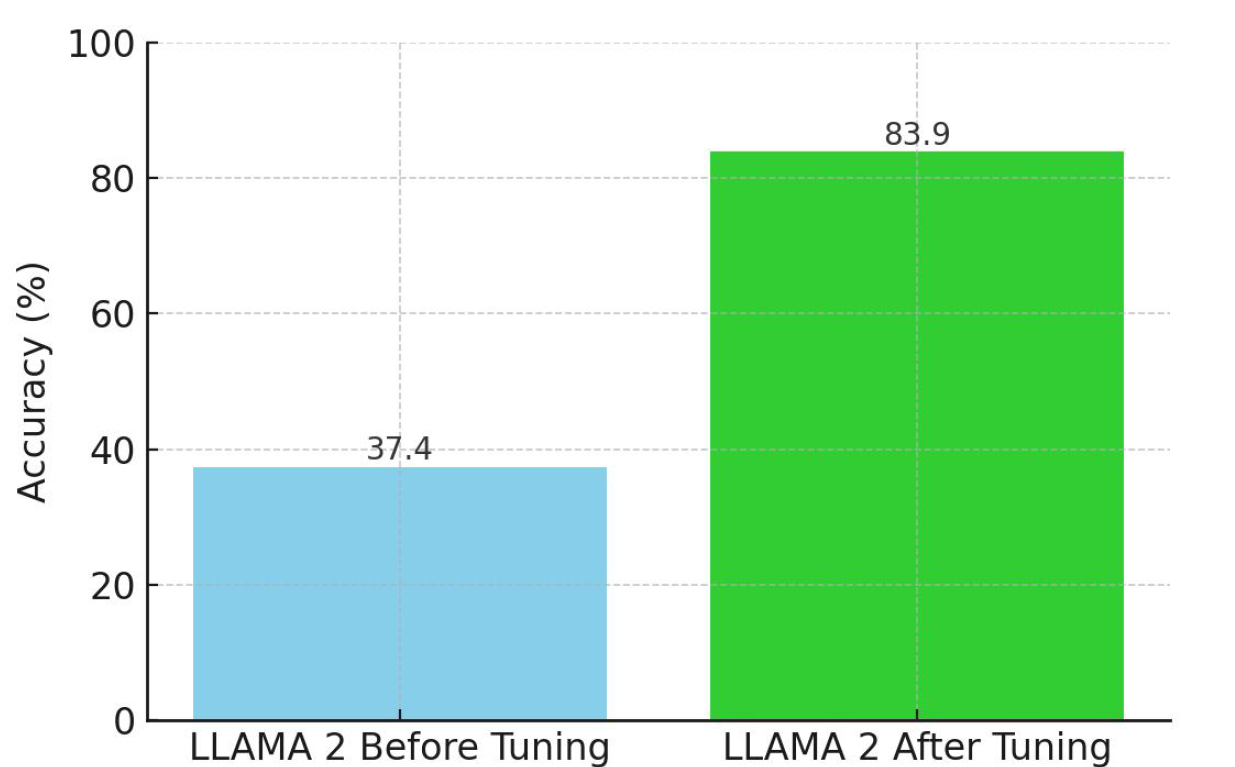
\includegraphics[width=1\linewidth]{fig1.png}
    \caption{\justifying \textit{Comparison of Model Accuracies}}
    \label{fig:FIG 1}
\end{figure}

LLAMA 2 initially demonstrated an accuracy of 37.4\%, which significantly improved to 83.9\% after fine-tuning. This marked enhancement underscores the importance of fine-tuning in optimizing model performance for sentiment analysis.

BERT, another transformer model, achieved an accuracy of 63\%. While it did not surpass the fine-tuned LLAMA 2, it still displayed a respectable level of accuracy.

\begin{figure}[H]
    \centering
    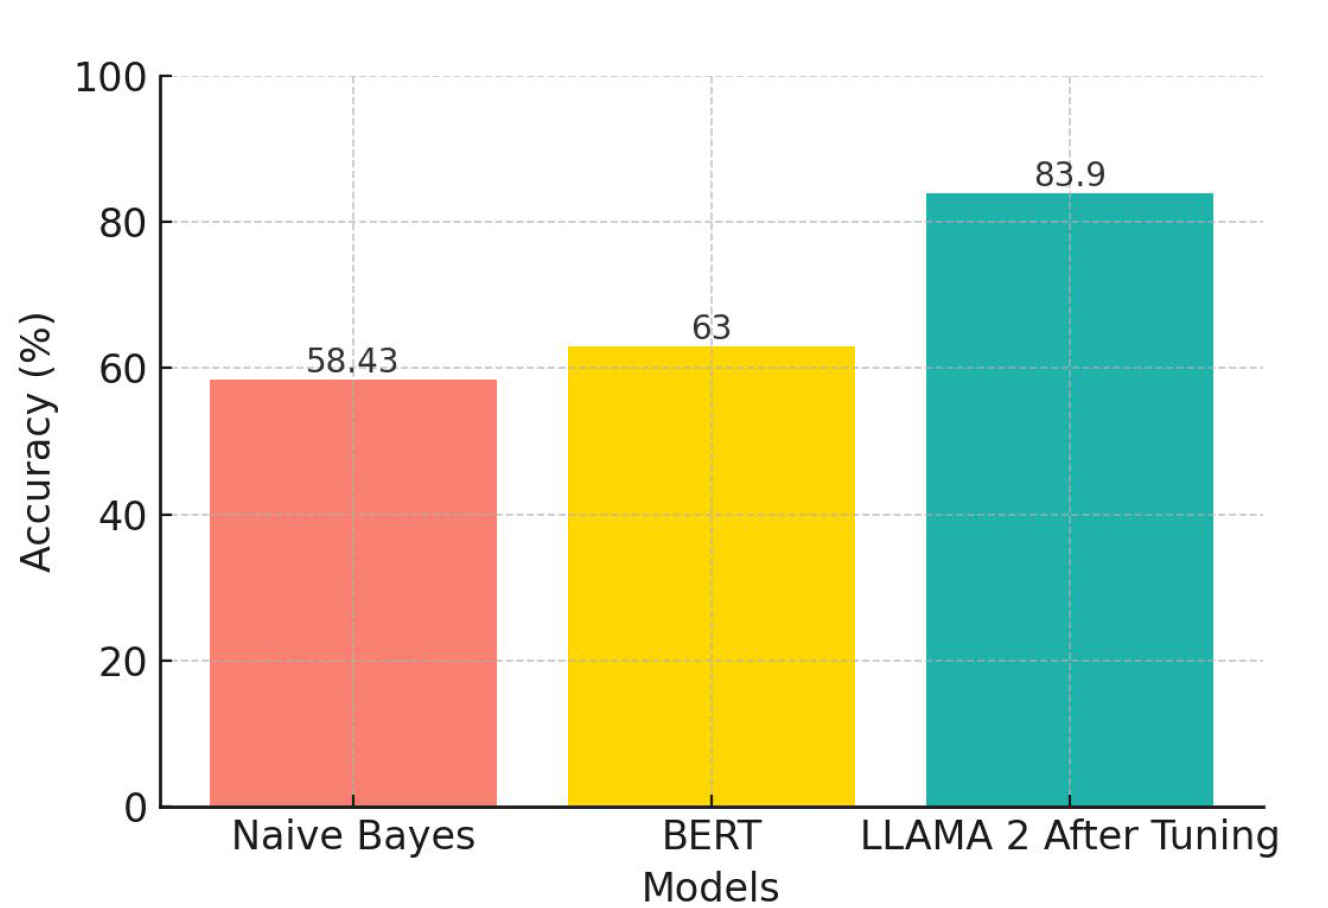
\includegraphics[width=1\linewidth]{fig2.png}
    \caption{\justifying \textit{LLAMA 2: Before and After Fine Tuning}}
    \label{fig:FIG 1}
\end{figure}

The effectiveness of these NLP techniques in sentiment analysis is evident in the visual comparison. The results emphasize the importance of model selection and fine-tuning, particularly for analyzing the complex dynamics of social media.

Furthermore, we compared the outcomes of our trained models with the results obtained by GPT-4 on political tweets. This comparison was aimed at assessing the congruence of our models with GPT-4 in the context of political sentiment analysis.

In this assessment, LLAMA 2 demonstrated an overall congruence rate of 40.4\% with GPT-4’s results in analyzing political tweets. The breakdown by sentiment categories revealed:
\begin{itemize}
    \item A 71.1\% congruence for negative sentiments.
    \item A notably low 0.11\% for neutral sentiments.
    \item A 50.7\% congruence for positive sentiments.
\end{itemize}

The particularly low congruence rate for neutral sentiments in LLAMA 2 may be attributed to our limited experience in fine-tuning NLP models. This suggests the potential for error or misclassification in this category, highlighting an area for further investigation and refinement in our approach.

The confusion matrix for the comparison with GPT-4’s results illustrates these disparities in more detail. While there is a relatively high number of agreements in the classification of negative sentiments, the discrepancies in the neutral and positive categories reflect the subjective nature of sentiment analysis and the diversity of approaches used by different models.

The congruence of our models with GPT-4's results offers a unique perspective on the reliability and consistency of sentiment analysis models. While some level of agreement is observed, particularly in certain sentiment categories, the disparities underline the need for further refinement and calibration of models for more consistent and accurate sentiment analysis, especially in diverse and complex datasets like those derived from social media.


\section{CONCLUSION}

This research has provided an in-depth analysis of various Natural Language Processing (NLP) models for sentiment analysis, particularly in the realm of political discourse on social media. Our study, primarily focusing on the Naive Bayes Classifier, LLAMA 2 (both pre- and post-fine-tuning), and BERT, has yielded significant insights into their capabilities and limitations in this context.

A key finding from our research is the notable impact of the fine-tuning process on model performance. The substantial improvement in LLAMA 2 post-fine-tuning highlights the potential of advanced NLP models to adapt to complex and nuanced data. However, it is important to acknowledge that our results could be influenced by the extent of our fine-tuning process and our relative inexperience in this specialized field. Despite these limitations, our study demonstrates that even with constrained resources, it is possible to develop effective methods for analyzing political sentiments on social media.

Our findings carry substantial implications for the political landscape. The ability to analyze social media sentiment accurately, even with limited resources, opens the door for individuals or groups with fewer resources to participate actively in political discourse. This democratization of sentiment analysis tools can level the playing field, allowing for a broader range of voices to be heard in the political arena, without the need for significant funding or influence from lobbyists and other vested interests.

However, there is a downside to consider. The advancement and accessibility of such NLP technologies also mean that foreign entities, including potentially adversarial nations, could employ these tools to monitor and potentially interfere in the political discourse of other countries. This capability presents a significant risk, as it allows external actors to gain a deeper understanding of the political climate and public opinion in targeted nations, potentially using this information to their advantage.

Future research should not only focus on refining these models and exploring the integration of various approaches but also consider the broader implications of their use, including ethical and security concerns. As we advance in our ability to understand and analyze political sentiments in the digital age, it is imperative to remain vigilant about the potential misuse of these technologies and to develop safeguards to prevent such scenarios.


\section*{Acknowledgments}

 We acknowledge the use of OpenAI's ChatGPT in refining the language and formatting of this paper. It is crucial to note that the core research, analysis, and conclusions within this document are entirely the work of the authors. Tools like ChatGPT were employed with discretion to enhance the clarity, coherence, and presentation of our narrative. This included assistance in language editing to ensure the paper is both accessible and academically rigorous.

\begin{center}
    \printbibliography[title={\fontsize{10}{12}\selectfont REFERENCES}, heading=bibintoc]
\end{center}


%\section{APPENDICES}





\end{multicols}

\end{document}
